\documentclass{llncs}
\usepackage{graphicx,soul,color}

%
\begin{document}

\title{Mass surveillance in cyberspace and the lost art of keeping a secret\thanks{The ideas discussed here first appeared as a DCSS project conference talk and were subsequently fleshed out in the form of a paper due to serendipitous encounters that were lovingly fostered by the social medium of Twitter.}}
\subtitle{Policy lessons for nation-states after the Snowden leaks}

\author{Theo Tryfonas\inst{1} \and Michael Carter\inst{2} \and Tom Crick\inst{3} \and Panagiotis Andriotis\inst{1}}
\institute{Crypto Group, University of Bristol, UK\\
\email {t.tryfonas@bristol.ac.uk, p.andriotis@bristol.ac.uk}
\and
Surveillance Studies Centre, Queen's University, Canada\\
\email{michael.carter@queensu.ca} 
\and
Dept. of Computing, Cardiff Metropolitan University, UK\\
\email{tcrick@cardiffmet.ac.uk}}

\maketitle

\begin{abstract}
Global security concerns, acts of terrorism and organised crime activity have motivated nation states to delve into implementing measures of mass surveillance in cyberspace, the breadth of which was partly revealed by the whistleblower Edward Snowden. But are modern nation states fighting a battle in the wrong space? Is mass surveillance of cyberspace effective and are the conventional metaphors of technology control appropriate for it? Can algorithms detect, classify and decide effectively on what constitutes suspicious activity? We argue that as cyberspace is a construct that has only recently been viewed strategically, let alone indoctrinated (the UK’s cyber-security strategy is only 4 years old), the societal impact of such bulk measures is yet much unclear – as are the assumptions about the fitness of state organisations that are charged with their oversight and the potential for unintended consequences. Recent experiences highlight the role of multiple forms of intelligence inputs, especially human- and community-based, and the need for application of such intrusive measures in a targeted manner. We believe that intrusive measures, where necessary, must be used decoupled from the seductive promises of advanced technology and ought to go hand-in-hand with means that strengthen the affected communities to identify, report and battle extremism and organised crime, in ways that safeguard the fundamental principles of our contemporary democratic Western states.
\keywords{Surveillance, cyberspace, public trust}
\end{abstract}

\section{Introduction}
\label{sec:Introduction}
In the fall of 2014, UN Special Rapporteur Ben Emmerson submitted his report on practices of mass surveillance by state actors and the threat that this approach to intelligence gathering poses to universal civil and political rights~\cite{Emerson}. Emmerson called for open and transparent discussion between government and citizens to inform and determine an appropriate balance between public security and personal privacy. The Special Rapporteur pointed out that what is technologically possible is not necessarily desirable or responsible. This is an argument that surveillance scholars such as Kirstie Ball have been making for several years now~\cite{Ball}. However, traction for this debate was limited until June 2013 when files leaked by NSA whistleblower Edward Snowden were published in the Guardian by journalist Glenn Greenwald.

Two years after the initial release of Snowden files, surveillance legislation remains highly contested in Canada, the US and the UK. Perhaps most notably is the sunsetting of section 215 of The Patriot Act and subsequent passing of The Freedom Act in the United States in early June 2015~\cite{Patriot}. Days later the Senate of Canada passed controversial anti-terrorism Bill C-51, which received sustained public opposition from big business, journalists, law professors, activists and the privacy commissioner~\cite{C-51}. A week prior to these developments the latest rendition of the so called 'snooper's charter' in the UK was announced in the Queen's speech. Former deputy Prime Minister Nick Clegg publicly opposed the legislation, currently known as The Investigatory Powers Bill, arguing it threatens the privacy rights of citizens. It's details are not fully fledged yet at the time of writing, but it is expected to be a contentious bill and Prime Minister David Cameron has at various points pointed towards banning the use of strong encryption -- albeit there would be fierce opposition to legislation against it. 

These measures are indicative of state attempts to curb terrorism threats by enabling the development of surveillance capabilities that are of bulk collection nature, rather than targeted to specific individuals. Proponents of these argue that the proliferation of high technology, including anonymity, cryptography and secure communication tools, enables organised crime and terrorists, extremists etc. to communicate safely and go undetected. On the other hand privacy activists advocate the fundamental need for safe spaces to develop one's ideas, the human right to privacy and an individual's need to protect themselves from abusive regimes.

In this paper we develop an argument about the place of mass cyberspace surveillance in society. We believe that deployment of intrusive systems on line, where necessary, should be of clear and transparent purpose to the public and accompanied by measures that empower the affected communities to tackle the root causes of concern, e.g. radicalisation, hate speech etc. Drawing on analogies from other surveillance systems we develop the idea of co-creation, in the civic innovation sense of the term, arguing that otherwise Western states risk developing non-transparent and unaccountable structures of power that undermine the fundamental values of their civilisation.

The rest of the paper is organised as follows: section~\ref{sec:Background} provides some further background to the issue of mass surveillance of cyberspace with an emphasis in the Anglo-Saxon West and discusses aspects of the Snowden leaks; section~\ref{sec:Understanding} develops some fundamental ideas and draws on analogies from other domains to explore the difficulties and challenges involved; section~\ref{sec:Creating} introduces our ideas and policy recommendations for a system-of-systems approach and co-creation of intrusive technologies; and finally we conclude with an overview section~\ref{sec:Conclusions}.

\section{Background}
\label{sec:Background}
The debate on mass surveillance, which is comprised of several threads, has engaged a range of social groups including politicians, law makers, journalists, academics, tech firms, activists, artists and the general public. The term mass surveillance is used to distinguish the bulk collection of data from targeted surveillance, which typically involves a 'person of interest'. Central to this aspect of the debate is the legal warrant, which is traditionally issued upon satisfaction of a certain level of suspicion. In the case of Canada, for example, Bill C-13, which was passed in the fall of 2014, significantly lowered the level of suspicion required to justify the collection of personal data. Bill C-13 also addressed the distinction between data and meta data, which is a hotly debated topic in surveillance legislation. In particular, Bill C-13 reduces the limitations on collecting meta data under the guise that it is not intrusive. Advocates of expanded surveillance powers for the state have attempted to mollify concerns by arguing that meta data does not threaten the political or civil rights of citizens because it is data about communication and not the content of communication. This argument has been routinely problematized by opponents who point out that metadata can reveal religious beliefs, political leanings and intimate relationships. Moreover, meta data is used by state actors to kill people, as was famously announced by former NSA and CIA director Michael Hayden~\cite{Hayden}. 

As legislation governing surveillance practices in Western society continues to evolve, a related debate is emerging. In early June, UN Special Rapporteur David Kaye submitted his report on the right to freedom of opinion and expression~\cite{Kaye}. Kaye argued that encryption and anonymity in digital communications is fundamental for the preservation of privacy and the protection of opinion and belief. The Special Rapporteur framed encrypted communication as a tool for citizens to protect their human rights from infringement by government agencies. Moreover, he called for the mobilization of state resources to ensure all individuals using digital communication can do so with encryption. Just prior to the release of the report, Nico Sell, co-founder of leading encryption app Wickr, launched a non-profit organization with this goal in mind. 

However, less popular apps like Wickr and more mainstream services like WhatsApp and Snapchat are being targeted by government. In January 2015 British Prime Minister David Cameron publicly announced his intention to ban communications that are not accessible by government agencies. Cameron asked for and quickly received support for this position from President Obama. The movement to ban encryption points towards the criminalization of private communication, which would threaten a variety of political, civil and human rights. Moreover, security experts have noted that weakening communication by demanding back door access will increase vulnerabilities and by extension could compromise national security. In May 2015 over 140 technology firms including Apple, Google and Symantec sent an open letter to President Obama urging him not to push for government access to encrypted communication. In the meantime, apps that offer individuals encrypted communication are proliferating as concern for privacy in mainstream society climbs.

\begin{figure}
\begin{center}
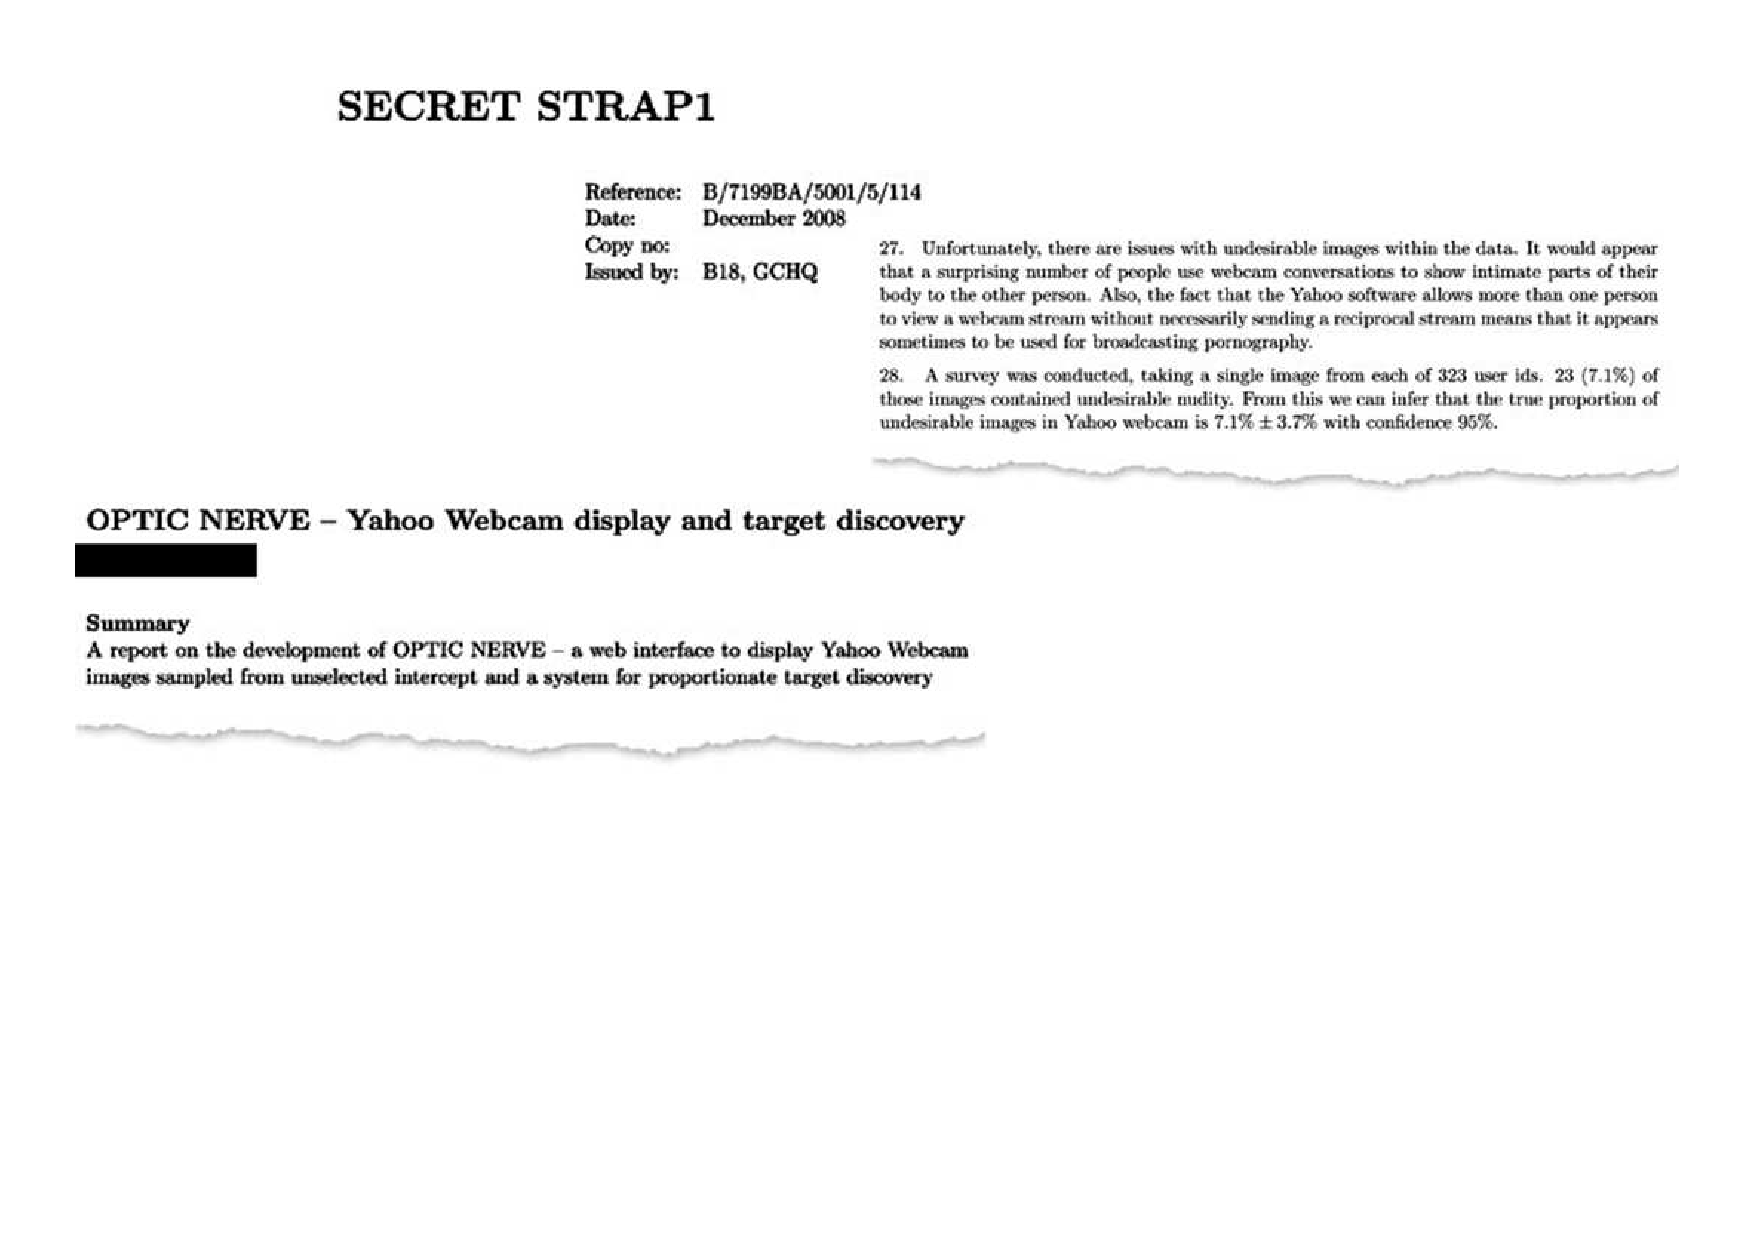
\includegraphics[scale=0.4]{fig1}
\caption{Yahoo! webcam traffic monitoring report snapshots from Snowden's cache.}
\label{fig:Yahoo}
\end{center}
\end{figure}

The Snowden leaks revealed a wide portfolio of projects and initiatives both from the NSA in the US, CSIS in Canada and GCHQ in the UK. These range from specific data collection projects such as Optic Nerve, aimed at Yahoo! webcam traffic (Figure \ref{fig:Yahoo}), to influencing the development of cryptographic standards to contain vulnerabilities, so they can be penetrated easier~\cite{ECDH}. In this varied context the Anderson report~\cite{Anderson} that was released recently as a comprehensive review of the UK's capabilities and practice prior to revamping the existing legislation, emphasised a number of issues, amongst the most important - and contested - of which, was the suggestion for judicial rather than ministerial oversight.

Politicians have already started countering the suggestion by claiming that despite the wide and varied nature of operations, ministers can have more topical information than judges and make decisions quicker, as opposed to going through the overheads of a judiciary procedure. However, due to the wide reach of operations it is questionable how much in depth understanding can law makers develop in the short amounts of time to decide in the absence of a transparent and well defined process. Another interesting point raised after the leaks is about the level of access and trust vested to a third-party, private contractor by security services, which may be indicative of the lack of resourcing of the relevant agencies -- and adding to the need for sufficient oversight.

\section{Developing public understanding of surveillance in the context of cyberspace}
\label{sec:Understanding}
\subsection{Deconstructing state imagery of cyber surveillance}
Politicians use many metaphors and analogies to promote the idea of cyberspace surveillance among the public. David Cameron, the UK Prime Minister, talked in early 2015 about the need for the state to be able to eavesdrop digital communications over the Internet, just as it can happen over the telephony network. Drawing on analogies between the more familiar phone technology and the public's understanding of a legitimate wire-tapping process, he tried to construct an image of accepted mass surveillance.

Another frequently used analogy is the case of the closed-circuit television (CCTV) surveillance systems. This is a familiar, and very tangible, system which in the UK at least enjoys large amounts of public tolerance and even approval~\cite{Ditton}, even at the face of lack of real evidence of its effectiveness~\cite{Woodhouse}. We will get back to this a bit later, discussing the experience of insitutionalisation of CCTV as a means of surveillance, particularly in the UK where it is widely deployed across the country.

Security services in turn have played a role in constructing further the popular image of surveillance in cyberspace. Firstly, they persist in disassociating bulk collection from mass surveillance and differentiating between metadata and content. This is an attempt to legitimise operations based by necessity on a wide scan surface dictated by the complex, interconnected nature of the Internet. In his valedictory speech at the Cabinet War Room on 21 Oct 2014, Sir Iain Lobban, previous head of GCHQ, having just assured that, of the huge volumes of information trafficked on-line, GCHQ were able to capture, store and process only a tiny amount, he went on to say:\\
\emph{``We access the internet at scale so as to dissect it with surgical precision. Practically, it is now impossible to operate successfully in any other way. You can't pick and choose the components of a global interception system that you like (catching terrorists and paedophiles), and those you don't (incidental collection of data at scale): it's one integrated system.''}~\cite{Lobban}

This reinforces the view of cyberspace surveillance as a wide surface scanning process (a Panopticon, as envisaged by Bentham in Figure \ref{fig:Panopticon}) followed by a clinical application of targeted algorithmics that would be able to pave the way for the more targeted content analysis by real people. The focus on metadata, bulk collection and automated processing before reasonable suspicion has been raised for a human to intervene, constructs an argument about this practice not constituting surveillance, in the sense of its warranted and targeted application.

\begin{figure}
\begin{center}
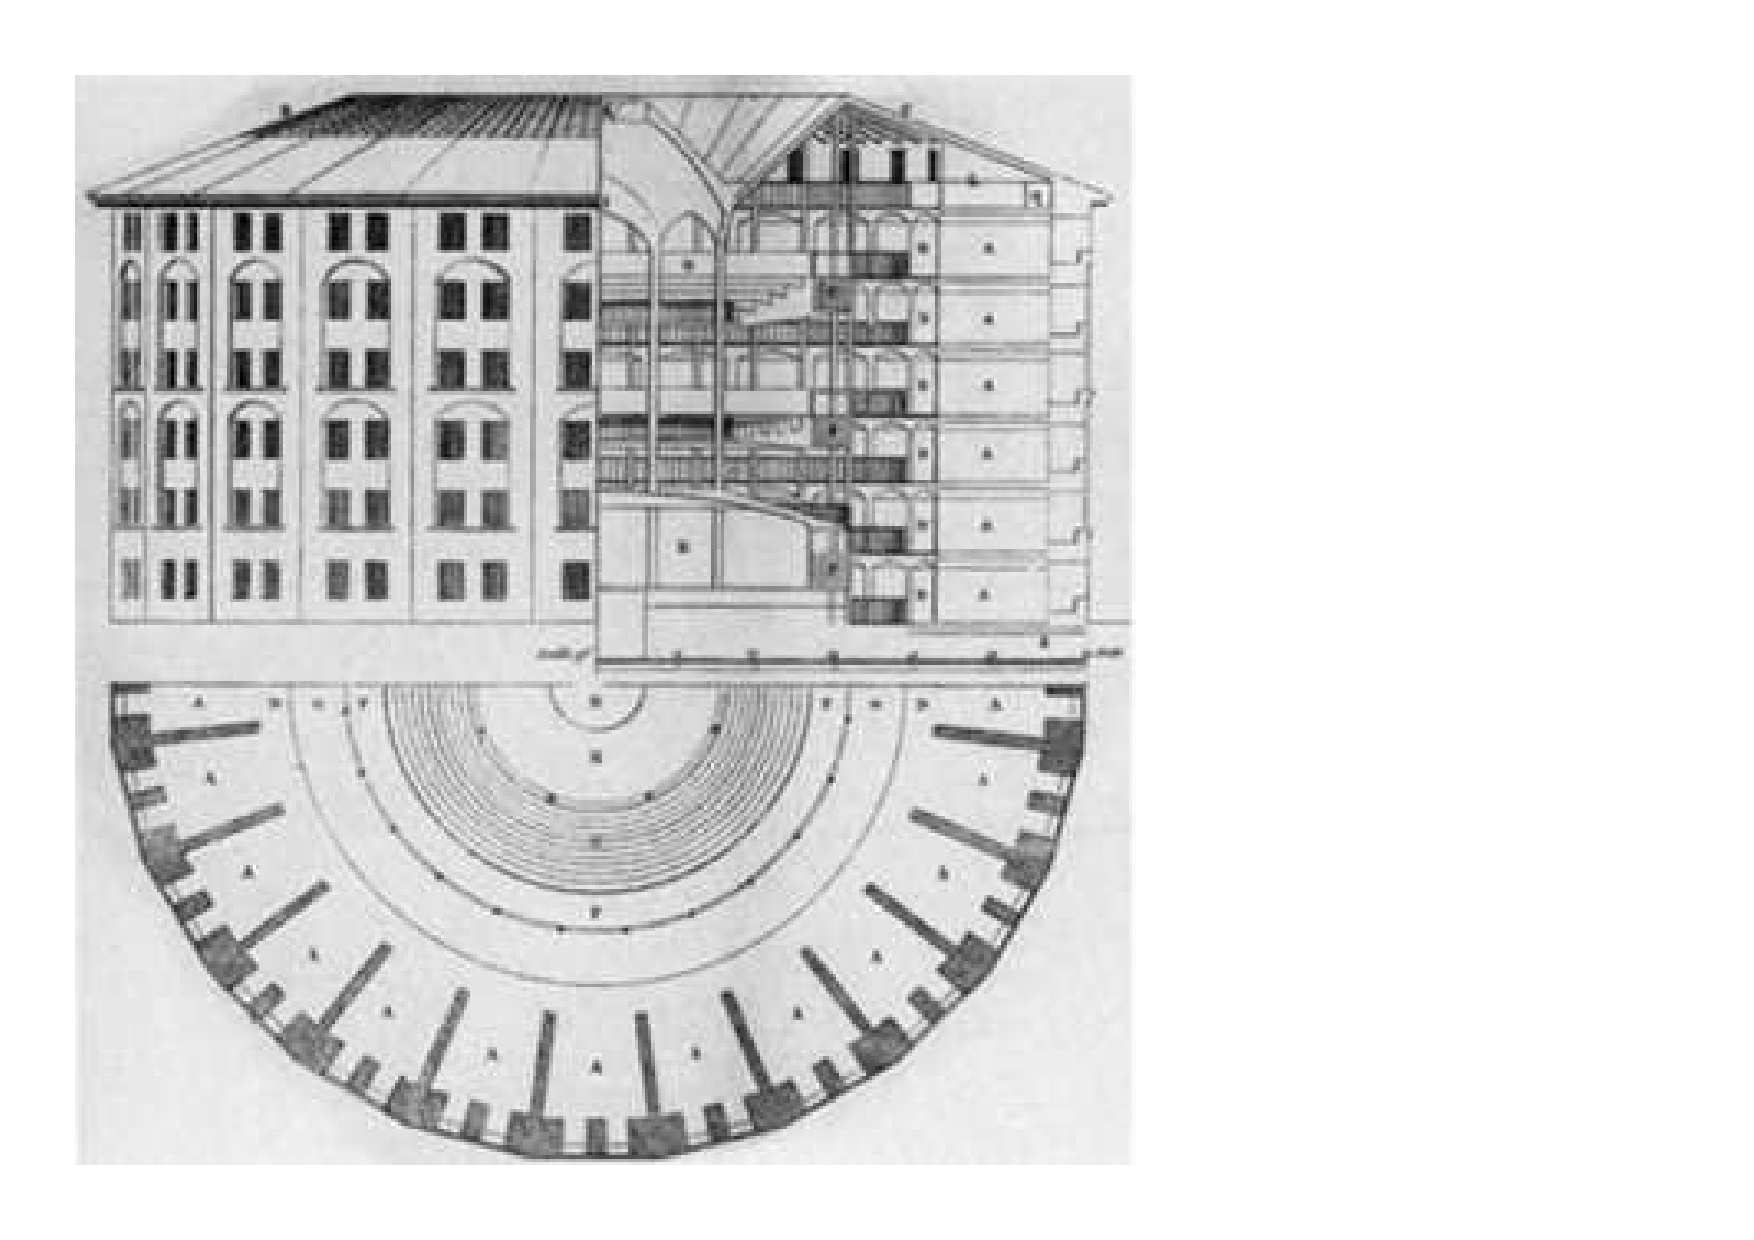
\includegraphics[scale=0.3]{fig2}
\caption{Part of Jeremy Bentham's designs for a Panopticon prison.}
\label{fig:Panopticon}
\end{center}
\end{figure}

Whether the Panotpicon metaphor matches the underlying security requirements is a significant question. This is because a metaphor is a conceptual construct able to shape action, as demonstrated by several scholars, including e.g. Tsoukas~\cite{Tsoukas}. Very soon after the attacks of 9/11, Lackoff argued that inappropriately framing the reaction as a 'war on terror' would produce unintended consequences~\cite{Lackoff}. Other research shows how secure systems implementation is shaped by the dominant security metaphors in use within organisations~\cite{Tryfonas}.

The Panopticon metaphor imposes the surveillance burden upon everyone, whether they are watched or not. This usually creates fundamental mistrust among many quarters of society towards government and the security services. But even viewed as bulk collection, it implies a huge sifting load for them. The report excerpts of Figure \ref{fig:Yahoo} demonstrate how the signal to noise ratio increases with bulk collection. The OPTIC NERVE programme was riddled with footage of genitals and posed significant challenges to intelligence officers as of how to handle the situation.

But the 'clinical' perception of the algorithmic component is problematic as well. Just as errors in human judgement may lead to tragic outcomes such as the shooting of Brazilian citizen Charles de Menezes in London by police in the aftermath of the 7/7 attacks, similarly algorithms may equally fail (the headline of Figure \ref{fig:Algo} is indicative of such a failure). In fact the absence of human judgement may cause this aspect to be perceived as even more untrustworthy. 

\begin{figure}
\begin{center}
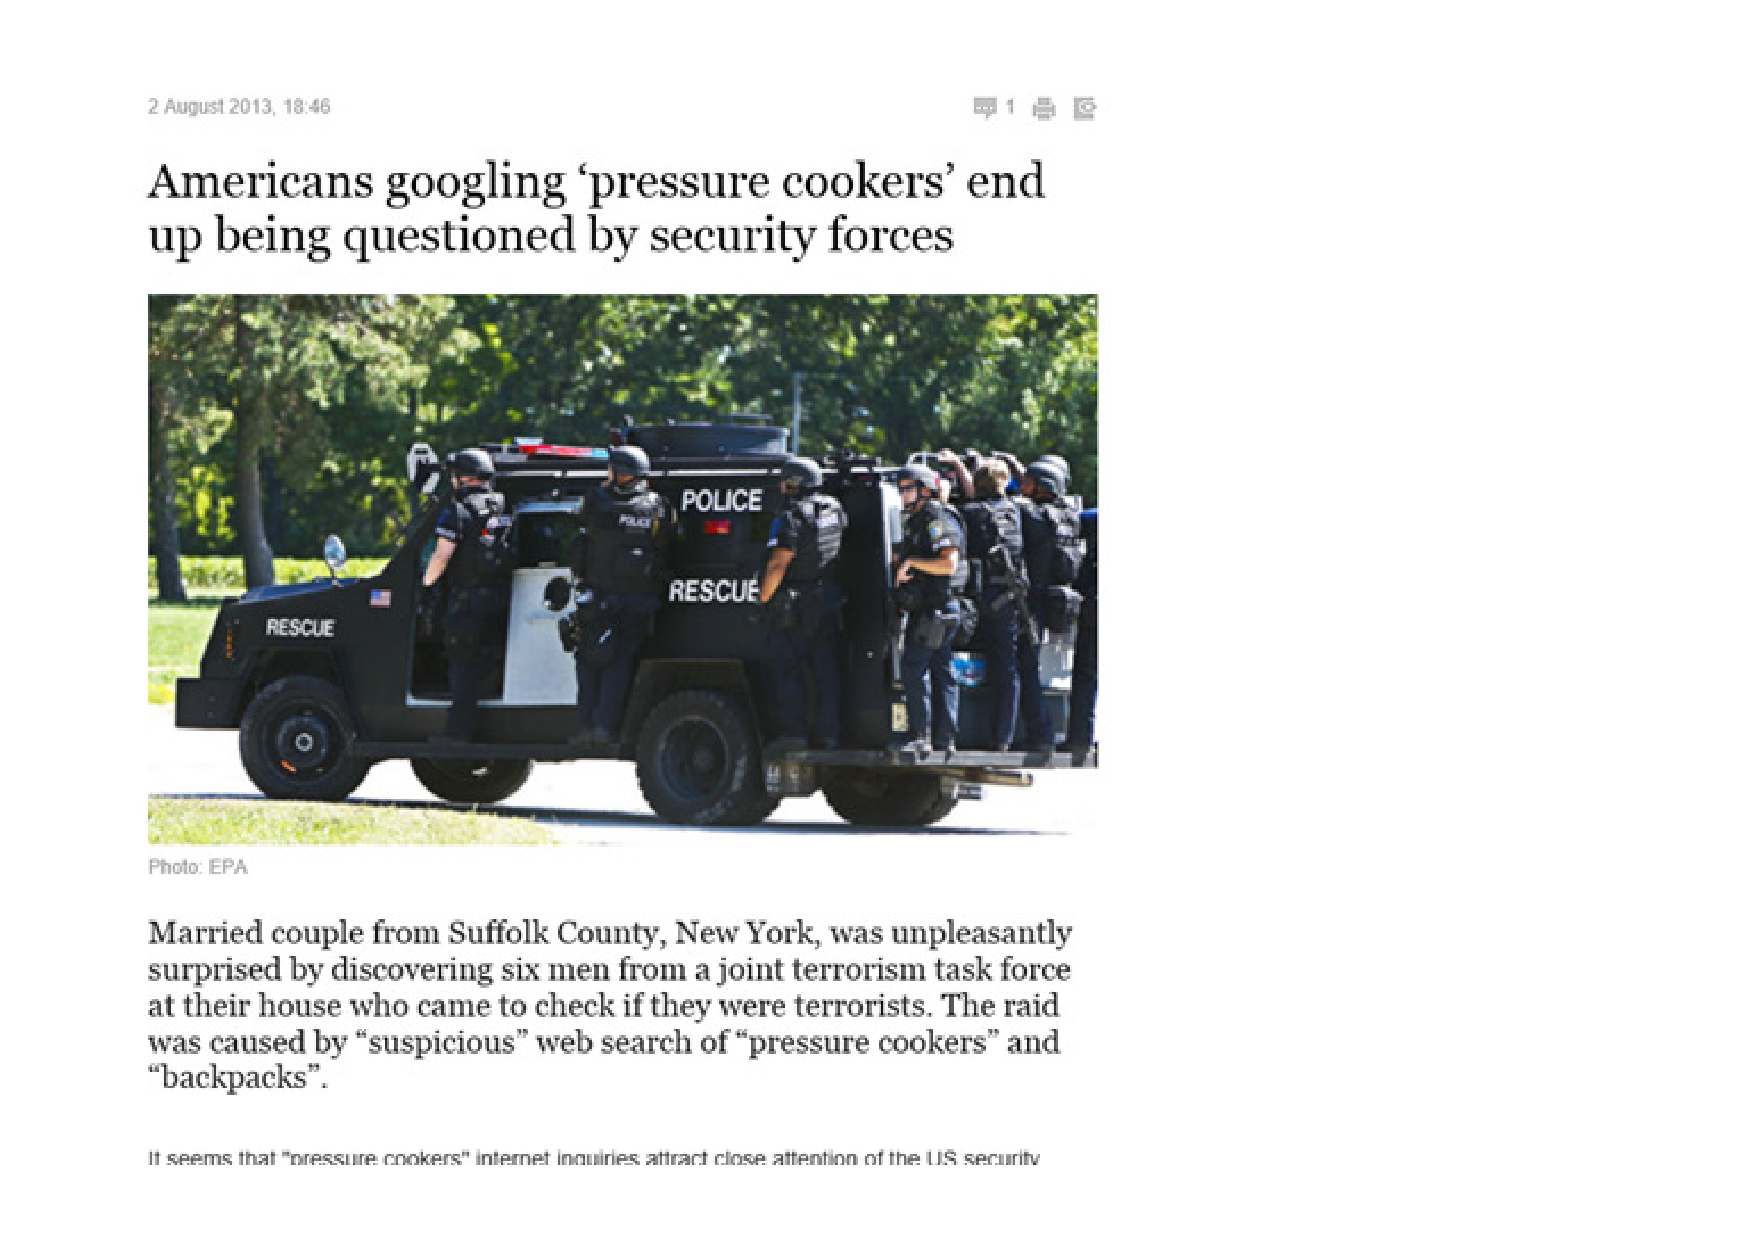
\includegraphics[scale=0.4]{fig3}
\caption{Failures of algorithmic determination after the Boston bombings.}
\label{fig:Algo}
\end{center}
\end{figure}

Another implicit assumption to legitimise this view is that this activity is organised under a framework of strong oversight. Particularly for the Anglo-Saxon world and especially for the UK, in the light of the strong leadership of prominent politicians such as Winston Churchill, Margaret Thatcher and Tony Blair, this assurance is almost taken for granted. However, history suggests that in the absence of oversight, socio-political circumstances may provide opportunity for exploitation of such structures. The experience of the rise of the Nazi party in the Weimar Republic is in line with this observation. Finally, we often also forget that the Internet is in reality a young technological development that it is yet much unexplored in terms of national security and military doctrine and use. The UK Cyber Security Strategy for example is less than 5 years old~\cite{Cyber}.

\subsection{Personal attitudes and the personal data dimension}
An interesting dimension of surveillance in cyberspace comes from the personal attitudes of the general public towards intrusive technology and its take up. Most recent disruptive innovations such as social networking platforms and wearable technologies are in fact privacy-intrusive by design. Computational paradigms that are based on the Cloud utilise lightweight computational intelligence of embedded systems and devices and harness the power of on-line servers to process large amounts of personal data. This 'commoditisation' of personal data happens on the trade off of personal service provision (e.g. wayfinding) in return for targeted advertising or aggregated consumer behaviour insight development that is then cashed in by the service provider, e.g. the GoogleAds model~\cite{GoogleAds}.

Despite the fact that providers of services such as Google and Facebook usually operate in multi-jurisdictions, which make difficult a coherent legislative approach and leave a lot of issues with respect to protection of personal data, there is a huge take up of their services. It seems that the personal value realised for each user, combined with the unclear implications/risks to the individual from their use have contributed largely to this. This is despite general concerns of legislators for their operation, as in the case of Belgium that investigated Facebook tracking of users, even when not logged in~\cite{facebookBel}. Also despite journalists and researchers have flagged how both in terms of practicalities such as extended data retention periods (e.g.~\cite{Wired}), but also how theoretically can be shown that providers tend to maximise their payoffs when they misuse personal data~\cite{Anastasopoulou}.

We argue that one of the side effects of this is the casualisation of attitudes towards privacy rights. There's a creeping indifference that could develop to passive acceptance through repeated interaction and use of such technologies -- in a way that Giddens describes as routinisation in his theory of structuration~\cite{Giddens}. However, familiarity with people giving up personal data in return for real value needn't necessarily be viewed negatively in the context of cyber surveillance. We will argue in the following section that such relationship can be at the centre of the creation of new surveillance systems, built upon consensus where intelligence is necessary and there is clear understanding of its value to all stakeholders.

\section{Co-creating viable surveillance systems}
\label{sec:Creating}

We referred earlier to CCTV as an example of a surveillance technology that has been relatively successful, from a technology acceptance and use point of view. That is particularly apparent in the UK, where it is estimated that there were over 4 million cameras in operation, although police investigations suggest that this may be an over-estimation~\cite{HomeOffice}. It is interesting to note that CCTV overall is really a collection of ad hoc installations of security cameras that offer access to footage of varying quality. These include public spaces monitoring as well as private surveillance systems for both corporate and personal property.

In reality CCTV is a system-of-systems that has emerged out of societal consent and adds some value (mostly evidential) to the law enforcement process. It is not standardised in terms of technical configurations or modes of operation, but of course its use is regulated, as personal data protection legislation applies. Notices of CCTV enforcement are for example mandatory to be displayed at the physical spaces that are monitored. Operators are also obliged to obfuscate streams that may be intrusive of personal space that could be accidentally included in the footage, e.g. certain frames that capture nearby windows. In Canada individuals may also be blocked out if they are in the frame and not directly relevant to an investigation. And in order to build public confidence, several operation centres in cities, such as traffic controllers, would include in their governance structures some involvement of members of the public, or elected local councillors.

Regardless of the heated debate about the effectiveness of CCTV against crime~\cite{Ditton}\cite{Woodhouse}, its proliferation and acceptance in some societies is notable. This is certainly the case in the UK, where CCTV rose to public prominence largely in the 80's. Part of its take up may be due to the campaign against football hooliganism as well as ground safety fears after the tragedy of Hillsborough. Some researchers also suggest that they became instruments of enforcing an image of a tough stance against crime by political parties, especially New Labour~\cite{McHill}.

The simplicity of purpose of a video surveillance system and the ability to relate its operation to a societal challenge (in this case football violence and public safety in grounds) established the technology in the collective social mind as something intrusive, yet necessary. This facilitated take up across public spaces of local councils (e.g. car parks), motorways, even on board means of transport, as well as in private business and buildings. Market forces and accessibility to the technology enabled everyone that may have had interest in it to install and operate such systems, creating space for the general public to serve as co-creators of the overall CCTV system-of-systems.

Translating this into the cyber domain, there is a need for related technology to be viewed as an enabler, as opposed to being demonised and fundamentally mistrusted. Greater transparency of Internet surveillance programmes and sufficient oversight structures would assure the public of the role of technology. Further education and public understanding of surveillance would help. This is not incompatible with the secrecy that security services claim must surround their operations; in fact they ought to assume that adversaries are suspicious of their practices. The Panotpticon metaphor needs to be revisited as until now it has blurred the realisation of the need to intervene earlier in the radicalisation lifecycle to debunk their propaganda messages and the appeal of radicalism to young and vulnerable members of society. There is a need for more human-centric intelligence, open source and targeted operations, as opposed to passive monitoring and algorithmic determination implied by the current paradigm. We believe that if the purpose is clear and the community is able to see the value to them, they will even tolerate the trade off of personal data in return for confronting effectively this threat, as suggested even by the commercial experiences discussed earlier.

\section{Conclusions}
\label{sec:Conclusions}
In light of global security challenges that include radicalisation and terrorism, but also increasing use of high technology by organised transnational crime, it is tempting for national states and their security services to develop mass surveillance programmes. The seductive promise of technological capability however, may not be a solution that is as relevant as human centric intelligence, as both wide surface scanning and artificial intelligence face their challenges as we've argued. And in any case this kind of capability is retrospective and missing the crucial stage of early intervention at the root cause of phenomena such as radicalisation of young persons to jihadist ideologies.

Creating powerful capabilities with insufficient oversight increases the potential for abuse of power and risks the loss of confidence and support from the wider public. This is exactly one of the aims of dissident groups and so we believe that organised states should refrain from developing surveillance capabilities in absentia of their key stakeholders, particularly the wider public. It is only with public trust that these may be successfully deployed. It is also essential that the paradigm of their development is one of a system-of-systems, i.e. viewed as an integral part of the wider state capability for countering terrorism and other organised crime. The whole picture ought to include early intervention to counter and debunk the appealing propaganda of terror groups and also to enable affected communities to report to, and cooperate with, the relevant authorities in confidence.

It is tempting for security services to explore every avenue of technology to counter such a severe threat. But the resulting programmes ought to respect fundamental rights of Western democracies, operate under strict due diligence and be accepted by the public, much like the example of CCTV in Britain. For, if the state in the process creates inadvertently the Matrix, it ought to be aware that the next historic revolution may come exactly from within it.

%
% ---- Bibliography ----
%
\begin{thebibliography}{}
%
\bibitem{Emerson}
Emerson, B.:
Annual report of the Special Rapporteur to the Human Rights Council, March 2014

\bibitem{Ball}
Ball, C.:
Organization, surveillance and the body: Towards a politics of resistance. In: Lyon, David ed. Theorising Surveillance: The Panopticon and beyond. Collumpton, UK: Willan Publishing. 

\bibitem{Patriot}
Kelly, E.:
Senate approves USA Freedom Act, Usa Today,  June 2, 2015

\bibitem{C-51}
House of Commons of Canada:
Bill C-51, first reading, January 30, 2015

\bibitem{Hayden}
Ferran, L.:
Ex-NSA Chief: 'We Kill People Based on Metadata', abcNEWS, May 12, 2014

\bibitem{Kaye}
Kaye, D.:
Report on encryption, anonymity, and the human rights framework, first report to the Human Rights Council, Office for the High Commissioner for Human Rights, 2015

\bibitem{ECDH}
Hales, T.:
The NSA Back Door to NIST, Notices of the AMS, Vol. 61, No 2, 191--192, February 2014

\bibitem{Anderson}
Anderson, D.:
A Question of Trust -– Report of the Investigatory Powers Review, Independent Reviewer of Terrorism Legislation, June 11, 2015

\bibitem{Ditton}
Ditton, J.:
Crime and the City, British Journal of Criminology, 40(4), 692-709, 2000

\bibitem{Woodhouse}
Woodhouse, J.:
CCTV and its effectiveness in tackling crime, House of Commons Library Standard Note SN/HA/5624 (2010)

\bibitem{Lobban}
Lobban, I.:
Sir Iain Lobban's valedictory speech - as delivered, GCHQ website, 2014

\bibitem{Tsoukas}
Tsoukas, H.:
The Missing Link: A Transformational View of Metaphors in Organizational Science, The Academy of Management Review, 16(3), 566-585, 1991 

\bibitem{Lackoff}
Lackoff, G.:
Metaphors of Terror, In: Return to The Days After, essays written in the aftermath of September 11, 2001, University of Chicago Press. 

\bibitem{Tryfonas}
Tryfonas, T.:
On Security Metaphors and how they shape the emerging practice of secure information systems development, Journal of Information System Security, 3(3), 21-50, 2007

\bibitem{Cyber}
UK Government:
The UK Cyber Security Strategy: Protecting and promoting the UK in a digital world, 2011

\bibitem{GoogleAds}
Google Inc.:
http://www.google.com/ads/

\bibitem{facebookBel}
Interdisciplinary Centre for Law and ICT/Centre for Intellectual Property Rights (ICRI/CIR), KU Leuven:
From social media service to advertising network: A critical analysis of Facebook’s Revised Policies and Terms, DRAFT 31 v1.2, March 2015

\bibitem{Wired}
Kravets, D.:
Which Telecoms Store your Data the Longest? Secret Memo Tells All. Wired Magazine, Sept. 2011

\bibitem{Anastasopoulou}
Anastasopoulou, K., Tryfonas, T. \& Kokolakis, S.:
Strategic stakeholder interaction analysis of cloud-based mobile applications use of privacy-sensitive end users, Lecture Notes in Computer Science, Springer, Vol. 8030, 209-216, 2013.

\bibitem{Giddens}
Giddens, A.:
The constitution of society: Outline of the theory of structuration. Cambridge: Polity Press. 1984. ISBN 0-520-05728-7.

\bibitem{HomeOffice}
Gerrard, G., Parkins, G., Cunningham, I., Jones, W., and Douglas, S.:
National CCTV Strategy. London: Home Office. 2007.

\bibitem{McHill}
McCahill, M. and Norris, C.:
CCTV in Britain Urbaneye, Working Paper no. 3. Centre for technology and Society, Technical University of Berlin. 2002.

\end{thebibliography}
\end{document}